\newpage
\section{Teilversuch 3: Spannungsabfall und Potentiometer}
Fehler bei dem Skalawert $\Delta x = 0,5$ Schritt\\
Fehler bei der Spannungmessung $\Delta U = 0,5\% \text{ Messwert} + 1$ Digit
\begin{equation*}
	\begin{tabu}{l *{11}{l}}
		\toprule
		\text{Skalawert $x/$Schritt} & 1000 & 900 & 800 & 700 & 600 & 500 & 400 & 300 & 200 & 100 & 0 \\
		\midrule
		\text{Helipot $U/\si{\volt}$} & 10,03 & 9,02 & 8,01 & 7,02 & 6,01 & 5,01 & 4,01 & 3,01 & 2,01 & 1,01 & 0,01 \\
		\text{Netzgerät $U_0/\si{\volt}$} & 10,03 & 10,03 & 10,03 & 10,03 & 10,02 & 10,02 & 10,02 & 10,02 & 10,02 & 10,02 & 10,02 \\
		\bottomrule
	\end{tabu}
\end{equation*}
Die Daten wurden mit \gnuplot{} geplottet und es wurde eine Kurvenanpassung zur $U = mx + c$ durchgeführt. Die entsprechenden Fehler sind im \gnuplot{} direkt berechnet. Für die genaue Rechnung, siehe Appendix \ref{appdx:gnuplottv3}. 
\begin{figure}[H]
	\centering
	% GNUPLOT: LaTeX picture with Postscript
\begingroup
  \makeatletter
  \providecommand\color[2][]{%
    \GenericError{(gnuplot) \space\space\space\@spaces}{%
      Package color not loaded in conjunction with
      terminal option `colourtext'%
    }{See the gnuplot documentation for explanation.%
    }{Either use 'blacktext' in gnuplot or load the package
      color.sty in LaTeX.}%
    \renewcommand\color[2][]{}%
  }%
  \providecommand\includegraphics[2][]{%
    \GenericError{(gnuplot) \space\space\space\@spaces}{%
      Package graphicx or graphics not loaded%
    }{See the gnuplot documentation for explanation.%
    }{The gnuplot epslatex terminal needs graphicx.sty or graphics.sty.}%
    \renewcommand\includegraphics[2][]{}%
  }%
  \providecommand\rotatebox[2]{#2}%
  \@ifundefined{ifGPcolor}{%
    \newif\ifGPcolor
    \GPcolortrue
  }{}%
  \@ifundefined{ifGPblacktext}{%
    \newif\ifGPblacktext
    \GPblacktexttrue
  }{}%
  % define a \g@addto@macro without @ in the name:
  \let\gplgaddtomacro\g@addto@macro
  % define empty templates for all commands taking text:
  \gdef\gplbacktext{}%
  \gdef\gplfronttext{}%
  \makeatother
  \ifGPblacktext
    % no textcolor at all
    \def\colorrgb#1{}%
    \def\colorgray#1{}%
  \else
    % gray or color?
    \ifGPcolor
      \def\colorrgb#1{\color[rgb]{#1}}%
      \def\colorgray#1{\color[gray]{#1}}%
      \expandafter\def\csname LTw\endcsname{\color{white}}%
      \expandafter\def\csname LTb\endcsname{\color{black}}%
      \expandafter\def\csname LTa\endcsname{\color{black}}%
      \expandafter\def\csname LT0\endcsname{\color[rgb]{1,0,0}}%
      \expandafter\def\csname LT1\endcsname{\color[rgb]{0,1,0}}%
      \expandafter\def\csname LT2\endcsname{\color[rgb]{0,0,1}}%
      \expandafter\def\csname LT3\endcsname{\color[rgb]{1,0,1}}%
      \expandafter\def\csname LT4\endcsname{\color[rgb]{0,1,1}}%
      \expandafter\def\csname LT5\endcsname{\color[rgb]{1,1,0}}%
      \expandafter\def\csname LT6\endcsname{\color[rgb]{0,0,0}}%
      \expandafter\def\csname LT7\endcsname{\color[rgb]{1,0.3,0}}%
      \expandafter\def\csname LT8\endcsname{\color[rgb]{0.5,0.5,0.5}}%
    \else
      % gray
      \def\colorrgb#1{\color{black}}%
      \def\colorgray#1{\color[gray]{#1}}%
      \expandafter\def\csname LTw\endcsname{\color{white}}%
      \expandafter\def\csname LTb\endcsname{\color{black}}%
      \expandafter\def\csname LTa\endcsname{\color{black}}%
      \expandafter\def\csname LT0\endcsname{\color{black}}%
      \expandafter\def\csname LT1\endcsname{\color{black}}%
      \expandafter\def\csname LT2\endcsname{\color{black}}%
      \expandafter\def\csname LT3\endcsname{\color{black}}%
      \expandafter\def\csname LT4\endcsname{\color{black}}%
      \expandafter\def\csname LT5\endcsname{\color{black}}%
      \expandafter\def\csname LT6\endcsname{\color{black}}%
      \expandafter\def\csname LT7\endcsname{\color{black}}%
      \expandafter\def\csname LT8\endcsname{\color{black}}%
    \fi
  \fi
    \setlength{\unitlength}{0.0500bp}%
    \ifx\gptboxheight\undefined%
      \newlength{\gptboxheight}%
      \newlength{\gptboxwidth}%
      \newsavebox{\gptboxtext}%
    \fi%
    \setlength{\fboxrule}{0.5pt}%
    \setlength{\fboxsep}{1pt}%
\begin{picture}(8640.00,5760.00)%
    \gplgaddtomacro\gplbacktext{%
      \csname LTb\endcsname%%
      \put(682,704){\makebox(0,0)[r]{\strut{}$-2$}}%
      \put(682,1332){\makebox(0,0)[r]{\strut{}$0$}}%
      \put(682,1960){\makebox(0,0)[r]{\strut{}$2$}}%
      \put(682,2588){\makebox(0,0)[r]{\strut{}$4$}}%
      \put(682,3215){\makebox(0,0)[r]{\strut{}$6$}}%
      \put(682,3843){\makebox(0,0)[r]{\strut{}$8$}}%
      \put(682,4471){\makebox(0,0)[r]{\strut{}$10$}}%
      \put(682,5099){\makebox(0,0)[r]{\strut{}$12$}}%
      \put(814,484){\makebox(0,0){\strut{}$-200$}}%
      \put(1875,484){\makebox(0,0){\strut{}$0$}}%
      \put(2937,484){\makebox(0,0){\strut{}$200$}}%
      \put(3998,484){\makebox(0,0){\strut{}$400$}}%
      \put(5059,484){\makebox(0,0){\strut{}$600$}}%
      \put(6120,484){\makebox(0,0){\strut{}$800$}}%
      \put(7182,484){\makebox(0,0){\strut{}$1000$}}%
      \put(8243,484){\makebox(0,0){\strut{}$1200$}}%
    }%
    \gplgaddtomacro\gplfronttext{%
      \csname LTb\endcsname%%
      \put(209,2901){\rotatebox{-270}{\makebox(0,0){\strut{}Spannung $U$ ($\si{\volt}$)}}}%
      \put(4528,154){\makebox(0,0){\strut{}Skala $x$ (Schritt)}}%
      \csname LTb\endcsname%%
      \put(7256,1482){\makebox(0,0)[r]{\strut{}$0,01001x + 0,00919$}}%
      \csname LTb\endcsname%%
      \put(7256,1196){\makebox(0,0)[r]{\strut{}Ausgangsspannung des Helipots}}%
      \csname LTb\endcsname%%
      \put(7256,910){\makebox(0,0)[r]{\strut{}Ausgangsspannung des Netzgeräts}}%
      \csname LTb\endcsname%%
      \put(4528,5429){\makebox(0,0){\strut{}Ausgangsspannung des Helipots gegen Skalenwerte des Helipots}}%
    }%
    \gplbacktext
    \put(0,0){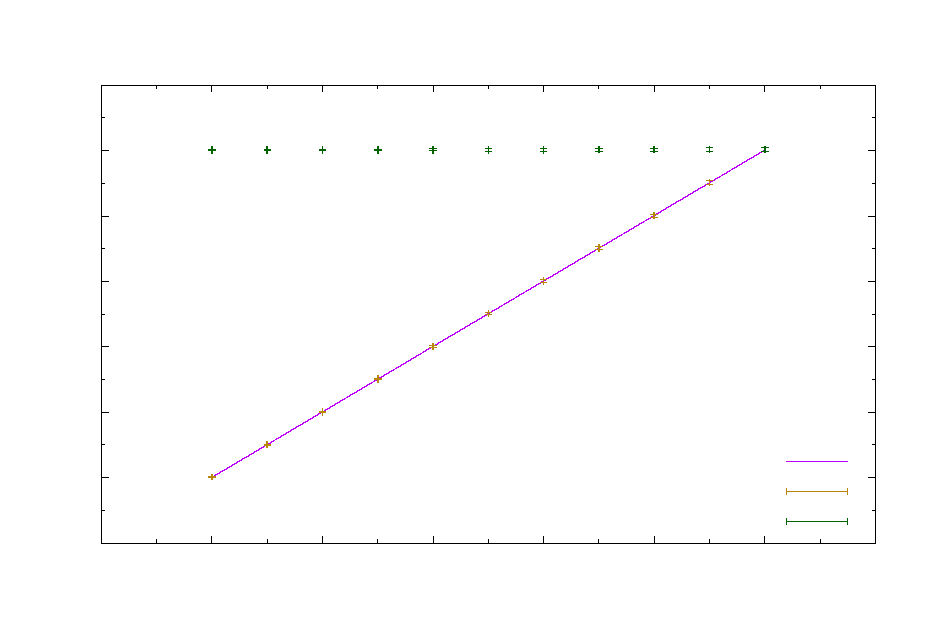
\includegraphics[width={432.00bp},height={288.00bp}]{tv3-plot}}%
    \gplfronttext
  \end{picture}%
\endgroup

	\caption{\centering Spannungsabfall im Abhängigkeit from Skalenwert des Helipots \captionbr $\chi^2_{\text{red}} = \num{0.0121338} \implies$ Gute Anpassung}
	\label{fig:tvthree-plot}
	\vspace{-1em}
\end{figure}
Als Endergebnis erhalten wir:
\begin{equation*}
	\begin{tabu}{lll}
		\toprule
		\text{Variable} & \text{Wert} & \text{Gerundet} \\
		\midrule
		m & \SI{0.0100079(33)}{\volt}~\text{Schritt}^{-1} & \SI{0.010008(4)}{\volt}~\text{Schritt}^{-1}\\
		c & \SI{0.009189(1003)}{\volt} & \SI{0.0092(11)}{\volt} \\
		\bottomrule
	\end{tabu}
\end{equation*}
Aus der Anleitung gilt aus
\begin{equation}
	R = \rho\frac{L}{A}
\end{equation}
dass
\begin{equation}
	U = \frac{x}{x_0}U_0 = \frac{U_0}{x_0} x
\end{equation}
Also ist die Spannung linear bezüglich $x$. Das ist tatsächlich was wir im Teilversuch 3(b) beobachtet haben. In Abbildung \ref{fig:tvthree-plot} ist diese lineare verhältnis klar veranschaulicht. 

Im Teilversuch 3(a) haben wir als Messungen:
\begin{equation*}
	\begin{tabu}{ll}
		\multicolumn{2}{l}{\SI{10}{\centi\meter} \text{ Messung}}\\
		\toprule
		\text{Messung 1} & \SI{0.615(5)}{\volt} \\
		\text{Messung 2} & \SI{0.607(5)}{\volt} \\
		\text{Messung 3} & \SI{0.613(5)}{\volt} \\
		\bottomrule
	\end{tabu}
\end{equation*}
Messungen 1 und 2 stimmt miteinander überein, und Messung 2 ist paarweise verträglich mit der anderen zwei Messungen, also ist die Spannungsabfall wie erwartet unabhängig davon, welchen Teil des Drahtes wir messen, sondern nur auf die Länge des gemessenes Teil. 

Weiterhin haben wir für verschiedene Länge die Spannungsabfall gemessen. Das Ergebnis ist auch wie erwartet: Der Spannungsabfall steigt linear mit zunehmende Länge, und zwar etwa $\SI{0,6}{\volt}$ je $\SI{10}{\centi\meter}$:
\begin{equation*}
	\begin{tabu}{ll}
		\toprule
		\text{Länge} & \text{Spannung} \\
		\midrule
		\SI{20.0(4)}{\centi\meter} & \SI{1.167(7)}{\volt} \\
		\SI{40.0(4)}{\centi\meter} & \SI{2.370(22)}{\volt} \\
		\SI{60.0(4)}{\centi\meter} & \SI{3.630(29)}{\volt} \\
		\SI{80.0(4)}{\centi\meter} & \SI{4.86(4)}{\volt} \\
		\SI{90.0(4)}{\centi\meter} & \SI{5.50(4)}{\volt} \\
		\bottomrule
	\end{tabu}
\end{equation*}
Es ist auch im Versuch 3(a) beobachtet, dass der Draht warm wird, wenn Strom durch ihn fließt. Das ist ein gutes Kennzeichen dafür, dass es einen Spannungsabfall im Draht gibt. Spannung ist Arbeit pro Ladung. In diesem Fall ist die Energie einer Ladung ins Wärme umgewandelt und somit entsteht einen Potentialdifferenz im Draht. Fühlt man keine wärme (bspw. in Bananenkabeln), dann gibt es oft auch keinen oder nur wenig Spannungsabfall im Draht. 

